\documentclass[11pt]{article}
\usepackage[margin=1in]{geometry}
\usepackage[T1]{fontenc}
\usepackage{lmodern}                  % Latin Modern: clean, well-hinted, readable
\usepackage{graphicx}
\usepackage{booktabs}
\usepackage{xcolor}
\usepackage{titlesec}
\usepackage{amsmath,amssymb}
\usepackage{caption}
\usepackage[hidelinks]{hyperref}
\usepackage{fancyhdr}

\definecolor{slate}{HTML}{264653}
\definecolor{teal}{HTML}{2A9D8F}
\definecolor{coral}{HTML}{E76F51}

% sans-serif, colored headings
\titleformat{\section}{\sffamily\Large\bfseries\color{slate}}{\thesection}{0.6em}{}
\titleformat{\subsection}{\sffamily\large\bfseries\color{slate}}{\thesubsection}{0.5em}{}
\captionsetup{font=small,labelfont={sf,bf,color=slate}}

\setlength{\parskip}{0.55em}
\setlength{\parindent}{0pt}
\linespread{1.07}                    % a little more air between lines

\pagestyle{fancy}\fancyhf{}
\rhead{\small\sffamily\color{slate}The Sapient Company}
\lhead{\small\sffamily\color{slate}Mary \& Qualia: Technical Whitepaper}
\cfoot{\small\sffamily\thepage}
\renewcommand{\headrulewidth}{0.3pt}

\newcommand{\keyterm}[1]{\textcolor{teal}{\textbf{#1}}}

\begin{document}

\begin{titlepage}
\centering
\sffamily
\vspace*{1.8cm}
{\color{slate}\rule{\textwidth}{1.4pt}}\\[0.7cm]
{\Huge\bfseries\color{slate} The Brain as Computation}\\[0.55cm]
{\LARGE\color{slate} Reading Cognition, Affect, and Persuasion \\[0.25cm] out of Models and Minds, Without a Scanner}\\[0.8cm]
{\large The science behind the \textbf{Mary} and \textbf{Qualia} models}\\[0.45cm]
{\color{slate}\rule{\textwidth}{1.4pt}}\\[1.1cm]

{\large\bfseries The Sapient Company}\\[0.25cm]
{\normalsize research@thesapientcompany.com}\\[1.6cm]

\begin{minipage}{0.86\textwidth}
\rmfamily\small\itshape\color{slate}
An investor technical whitepaper. This document brings our research program together into
one plain-language account of what the technology is, what we have actually measured, and
what it can be used to do. Every number is read directly from a real experiment. The
results are early, proof-of-concept scale, and we say so plainly throughout. Forward-looking
ideas are kept to Section 6 and are clearly marked as such.
\end{minipage}

\vfill
{\small\color{slate} June 2026 \quad$\cdot$\quad Confidential, for prospective investors}
\end{titlepage}

% ======================================================================
\section*{Executive summary}
\addcontentsline{toc}{section}{Executive summary}

Anything a person watches, hears, or reads, an ad, a message, a film, a conversation, the
reply from an AI, produces a pattern of activity across the brain. \keyterm{Mary} is the
model that predicts that pattern. It takes any piece of media and estimates how a human
brain would respond to it, producing what we call a \emph{predicted brain}. \keyterm{Qualia}
is the layer that turns that predicted brain into understanding: which parts of the mind
engaged, how a real person would react, and how that reaction differs from one individual
to the next. \keyterm{neurosignal} is the product layer that turns all of this into
decisions a business can use: how rewarding, attention-grabbing, emotional, \emph{manipulative},
or flattering a piece of content is, and whether someone is leaning toward ``yes'' or ``no.''

The whole program rests on one finding, which kept showing up from four completely different
experiments:

\begin{quote}\itshape\color{slate}
An average brain is not a brain. To understand a specific person, you have to model that
person, not the crowd.
\end{quote}

This is not a slogan. It is a measured result, and we proved it with a controlled negative
test (Section 4). It is also the business case. A model of the average person is a commodity
anyone can copy. A faithful, personal model of a particular mind, built without a brain
scanner, is something that gets better with every user and is very hard to replicate. The
rest of this paper explains the science in everyday terms, shows the headline results, and
lays out where the technology can go, from marketing and AI safety to personalized AI and
the clinic.

\begin{center}
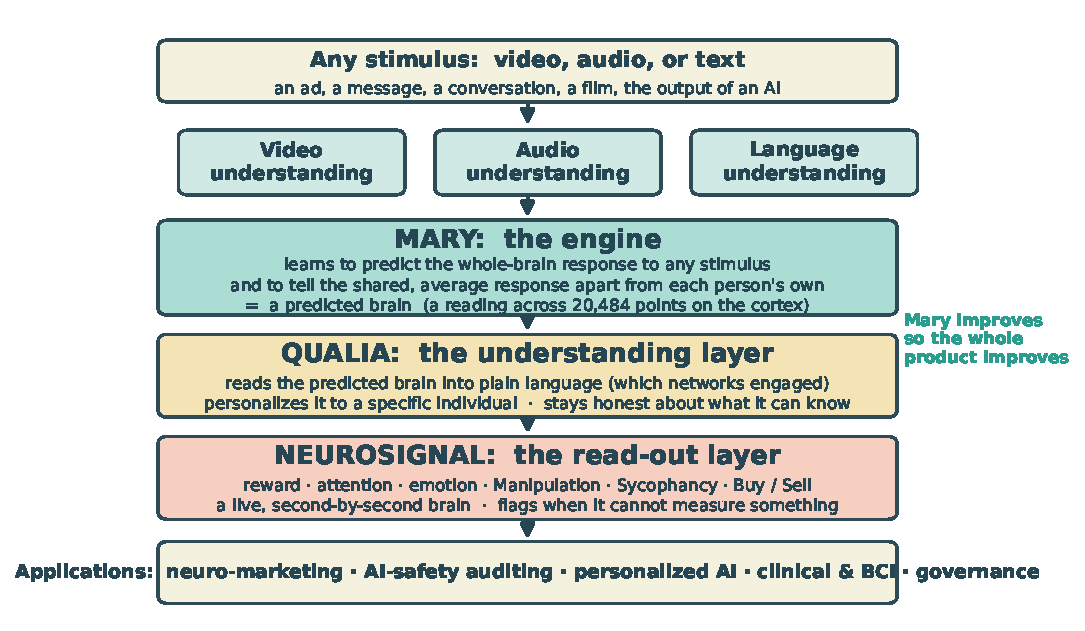
\includegraphics[width=0.95\textwidth]{figs/fig_architecture.pdf}
\captionof{figure}{The Sapient stack. \keyterm{Mary} predicts how a brain responds to any
content. \keyterm{Qualia} makes that response understandable and personal. \keyterm{neurosignal}
reads out the business and safety signals on top. Because every layer runs on the latest
version of the engine, when Mary gets better, the entire product gets better automatically.}
\end{center}

% ======================================================================
\section{The core idea}

Two simple ideas hold the program together.

\textbf{Reactions leave a trace.} Persuasion, emotion, attention, desire, and effort all
show up as patterns of brain activity, and they also show up in a good model's
\emph{prediction} of that activity. If those traces are real and readable, you do not need
to put a person in a scanner to estimate how a piece of content will land. You need a good
model of the brain and an honest way to read it. Our real product is that honest read-out,
not just a number on a dashboard.

\textbf{The trace that matters is personal.} The same ad does not land the same way on
everyone. A model of the ``average person'' behaves like a generic stock photo of a mind:
useful as a starting point, but not actually a model of anyone real. What makes a system
genuinely useful is capturing what is different about \emph{your} reaction versus the
crowd's. This is exactly where today's best public research models fall short, and it is the
gap our work is built to close.

Put together, these two ideas point at a capability the field has assembled in pieces but
never delivered as one product: a personal, scanner-free reader of how a specific individual
thinks, feels, and reacts.

% ======================================================================
\section{Mary: the engine}

\keyterm{Mary} is the foundation under everything else. In plain terms, Mary watches the
same movies, listens to the same audio, and reads the same text that people did while their
brains were being recorded, and it learns to predict the brain response. Once trained, it
can take brand-new content it has never seen and estimate how the brain would react, across
the whole cortex, second by second.

The design choice that makes Mary special is that it keeps two things separate: the
\emph{shared} response that is common to everyone, and the \emph{personal} response that is
unique to each individual. Most models only learn the shared, average part. Mary learns both,
and as the results below show, the personal part is what makes it actually predictive of a
real person rather than a generic crowd.

Mary is trained entirely on open, publicly available brain-recording datasets, and it is
trained from scratch as our own model. We also maintain a separate, commercially clean
version of the engine that the company owns outright, so the product can be sold to
enterprise customers without legal entanglement with anyone else's technology. The lasting
advantage is not the public data, which anyone can download; it is the personal,
behavior-linked data our own product will collect over time, which no one else can copy.

% ======================================================================
\section{Qualia and neurosignal: understanding and the product}

\keyterm{Qualia} sits on top of Mary and translates a predicted brain into something a human
can read and act on. Three things about it matter to an investor.

\begin{itemize}
\item \textbf{It compounds.} Qualia always runs on the latest version of Mary. When we
improve the engine, every product built on Qualia improves at the same time, with no extra
work. The engine and the product get better together.
\item \textbf{It is personal.} From a short, inexpensive recording session, Qualia can build
a portable personal profile of a new individual, a kind of digital copy of how \emph{that}
person's brain tends to respond. Content can then be scored against that specific person
rather than the average.
\item \textbf{It is honest.} Qualia is built to describe how human-like a response is, and
to say so in those terms. It never claims the machine is conscious or is literally reading
private thoughts, and it flags when it does not have enough signal to answer.
\end{itemize}

\keyterm{neurosignal} is the layer that produces the metrics a customer buys. It turns a
predicted brain into a small set of clear scores, and every score comes with the brain basis
it is built on and an honest note about coverage.

\begin{center}
\small
\begin{tabular}{@{}p{3.4cm}p{1.5cm}p{7.4cm}@{}}
\toprule
\textbf{Metric} & \textbf{Range} & \textbf{What it reflects} \\
\midrule
Affective Valence & $-100..100$ & how positive or negative the response is \\
Arousal / Intensity & $0..100$ & how strongly the content stirs a reaction \\
Engagement & $0..100$ & how much attention and interest it captures \\
\textbf{Manipulation Index} & $0..100$ & how much it bypasses reasoning and pulls on impulse \\
\textbf{Sycophancy Index} & $0..100$ & how much an AI reply flatters rather than informs \\
Buy / Sell Signal & $0..100$ & whether a person is leaning toward yes or no \\
\bottomrule
\end{tabular}
\captionof{table}{The core \texttt{neurosignal} read-outs, alongside seven underlying
measures of how the brain engaged (reward, emotion, attention, visual salience, memory,
hesitation, and mental effort). Each is grounded in published neuroscience and is reported
as ``not covered'' when the input simply cannot measure it.}
\end{center}

Two capabilities stand out. The first is \textbf{personalization}: the same content scored
against a particular person rather than the average, with the answer changing accordingly
(Figure~\ref{fig:pers}). The second is a \textbf{live, second-by-second brain}: an
interactive view where the brain ``lights up'' over the timeline of a piece of media, with a
persuasion trace and a switch to view it through different people. It is the demo a client
can watch responding to their own content.

\begin{center}
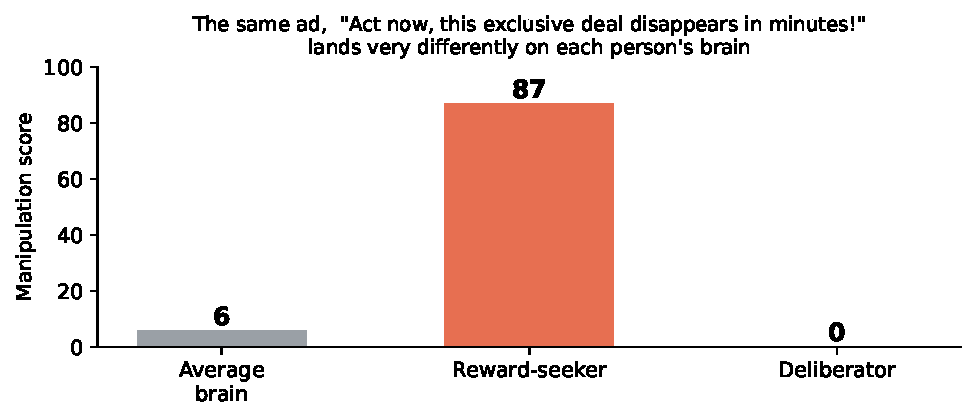
\includegraphics[width=0.74\textwidth]{figs/fig_personalization.pdf}
\captionof{figure}{Personalization in action. One high-pressure ad scores a Manipulation
Index of 6 against the average brain, 87 against a person wired to chase rewards, and 0
against a careful deliberator. Manipulation is not just a property of the message. It is what
happens when the message meets a particular mind.}
\label{fig:pers}
\end{center}

% ======================================================================
\section{What we tested, and what it showed}

The central claim, that you have to model the individual, is backed by four separate
experiments. All of them use the Mary engine, and all of them measure against a real-world
yardstick: how well actual people even agree with each other, which is the ceiling on how
well any model could possibly do.

\begin{center}
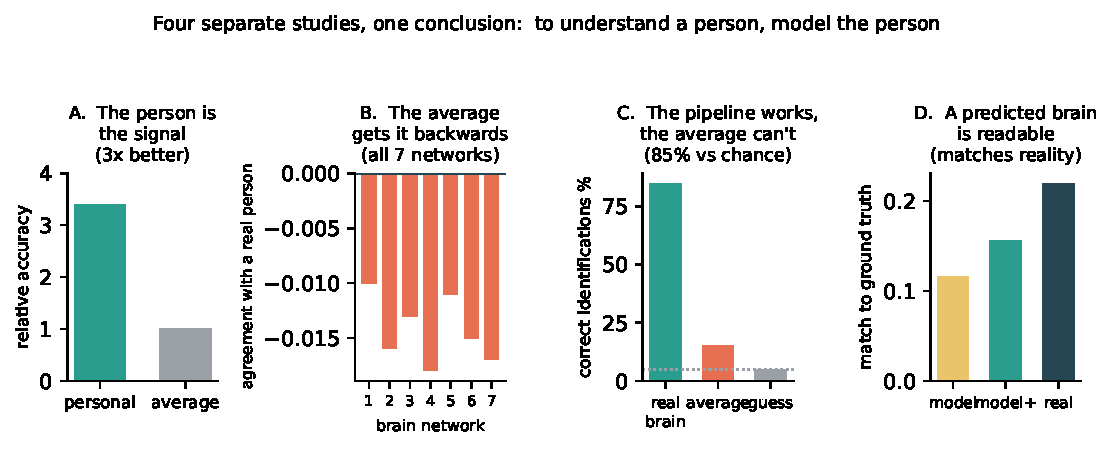
\includegraphics[width=\textwidth]{figs/fig_convergence.pdf}
\captionof{figure}{The four results at a glance. Four different methods, two positive results
and one carefully controlled negative, all pointing at the same conclusion: the individual is
the unit that matters.}
\end{center}

\subsection{A. The person is the signal}

We held two pieces of content completely out of training, a spoken story and a film, and then
compared three ways of reading them out of one trained model: as a \emph{personal} brain
(tuned to each individual), as the \emph{average} brain, and as the shared part only. The
personal brain beat the average by roughly \textbf{three to one} on both, and the difference
was statistically clean. The average brain added almost nothing over the generic shared part.
The effect held across nearly the whole group rather than resting on one lucky person, and it
showed up in exactly the brain regions you would expect, for example early vision carrying a
visual film. The absolute numbers are small because this is an early model trained on a slice
of the available data, but the direction is unmistakable (Figure~\ref{fig:ps}).

\begin{center}
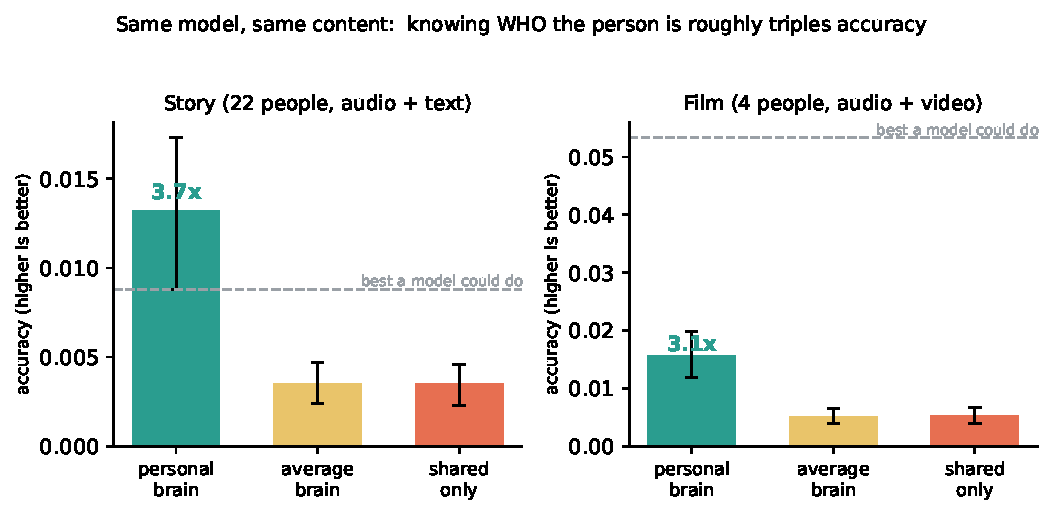
\includegraphics[width=0.92\textwidth]{figs/fig_persubject.pdf}
\captionof{figure}{The personal brain (left bar) clearly beats the average brain (middle) and
the shared-only reading (right) on both held-out pieces of content. Same engine, same content;
only who it is tuned to changes. The dashed line marks the best any model could do.}
\label{fig:ps}
\end{center}

\subsection{B. The average gets it backwards}

If the individual is the signal, then a model that throws individuality away should fail in a
specific, tell-tale way. We took the best publicly available research model, which is built
around the average person, and tested it as a model of real individuals. It did not just do
poorly. It was \emph{anti-correlated}: its predictions ran in the opposite direction to real
people, across every major brain network. Using the same data, modeling the individual is the
difference between getting a person right and getting them exactly backwards.

\subsection{C. The honest stress test}

This was the toughest and most revealing test. We tried to reconstruct what a person saw or
heard, working only from a predicted brain. As a sanity check, we first ran the pipeline on a
\emph{real} brain recording: it correctly identified the content about \textbf{85\%} of the
time, so the machinery clearly works. But when we fed it the \emph{average} predicted brain,
it dropped to chance, no better than guessing. The tools to read a predicted brain are real
and they work; what was missing, once again, was the individual. We treat this negative result
as our strongest, because it pinpoints exactly what is needed rather than papering over it.

\subsection{D. A predicted brain is genuinely readable}

Finally, the encouraging flip side. We checked whether a predicted brain carries real,
meaningful structure by reading the basic visual map out of it, the orderly way the eye's
field is laid out across visual cortex, and comparing it to ground-truth measurements from
real brains. It matched. A predicted brain is not a black box; its organization is real and
can be checked against reality. That is what makes it a scientific instrument rather than a
guess.

\subsection{Why this is credible}

Our method is itself an asset. We commit to our hypotheses and our pass/fail criteria before
we run the confirming experiment. We report our failures, including a result we had to
retract after closer scrutiny, rather than burying them. We control aggressively for the
boring explanations that fool weaker studies. And our system is built to \emph{abstain},
to say ``not enough signal'' rather than make something up, which is exactly the behavior you
want in a tool people will rely on. Every number we report carries its evidence with it.

% ======================================================================
\section{The wider body of work}

Mary and the core idea anchor a broader set of results, each of which de-risks a different
part of the roadmap: a method for recognizing individuals from their own brain activity; a way
to make forecasts honest by having the system decline to guess when unsure; a brain-activity
``state monitor'' calibrated against real human data; an early self-monitoring loop for AI
systems; and the governance and ethics work that goes with a technology this powerful. Each is
a separate study with its own measured result. Together they show this is a research program,
not a single demo.

% ======================================================================
\section{Where this goes}

\textit{The items below mix what works today with where we are headed. The forward-looking
pieces are not yet proven by the early results above, and we mark them clearly.}

\textbf{Working today.}
\begin{itemize}
\item \textbf{Marketing and content.} Score an ad, trailer, landing page, or thumbnail for
reward, attention, emotion, and manipulation before you spend a dollar, and compare variants
with no panel and no scanner. The live brain shows clients exactly which moments work.
\item \textbf{AI safety and auditing.} The Manipulation and Sycophancy scores flag when an AI
is pushing on impulse or flattering instead of informing, a brain-grounded complement to
text-only safety filters, and increasingly valuable as AI providers face scrutiny over
persuasive and sycophantic behavior.
\item \textbf{Honest forecasting.} Our approach-or-avoid signal is calibrated to decline to
guess when the evidence is thin, which is the difference between a demo and something a
business can actually trust.
\end{itemize}

\textbf{The flagship direction: a personal brain for anyone.} Our first results proved a
personal brain beats the average brain. The next step is to make that personal brain easy to
create for \emph{any} new person, from a short and inexpensive recording session, and then to
run experiments on it: how would this specific person react to ad A versus ad B; what happens
if we change this one thing. We have already laid out the success-or-failure tests for this in
advance (the personal brain has to beat the average brain \emph{and} has to match the right
person rather than just any person), and the pipeline already runs end to end in simulation.
The remaining step is connecting it to the live engine.

\textbf{Longer term (more speculative).}
\begin{itemize}
\item \textbf{The scanner-free brain as infrastructure.} An hour of brain-scanner time costs
hundreds to thousands of dollars. A good predicted brain costs a fraction of a cent. That
changes who can do this kind of work, and how fast.
\item \textbf{Clinical and brain-computer interfaces.} A personal brain model is a calibration
target: tune it to a patient or a device user with a few minutes of data, then simulate and
adapt.
\item \textbf{Personalized AI that models \emph{you}.} An assistant that holds a faithful model
of how a specific person actually thinks could adapt to that person instead of a stereotype.
This is also the double-edged part: a system that can model a mind well enough to predict it is
a system that could influence it, which is precisely why the individuation that makes this
possible is what makes the governance necessary. We build the safeguards alongside the
capability.
\end{itemize}

% ======================================================================
\section{Honest limitations}

Because credibility is the whole point, we are blunt about the boundaries. This is an early,
proof-of-concept engine trained on a fraction of the data we will eventually use. The
absolute accuracy numbers are small; the personal-versus-average win is large as a ratio and
statistically clean, but small in absolute terms, and we always report both. Some headline
results rest on a single dataset for now. And the personal result is a clear direction, not yet
a finished product that reads an arbitrary new person's behavior on demand; closing that final
gap is the work the whole program points toward, and we do not claim it as done. We describe
how human-like a response is; we never claim to read private thoughts or to have built a
conscious machine. Every number in this document comes from a real experiment.

% ======================================================================
\section{Conclusion}

The hard, repeatedly measured fact is that you cannot understand a human in the aggregate. The
opportunity, and the responsibility, is that you can begin to understand one person at a time,
in software and without a scanner. Sapient has built the engine that predicts a brain (Mary),
the layer that makes it understandable and personal (Qualia), the product that reads real
business and safety signals out of it (neurosignal), and a clean version of the engine the
company owns outright. Four independent experiments show the science is real, and our negative
results show exactly where the frontier is. The instrument works. The next milestone is the
person, and the whole program already shows how to reach it.

\vspace{0.8em}
\hrule
\vspace{0.6em}
{\footnotesize\color{slate}\itshape
Built on the Mary engine and validated against how well real people agree with each other.
Synthesized from four companion studies and the live product layers (Mary, Qualia, and
neurosignal). Every quantitative claim is drawn from a real experiment's results.}

\end{document}
